\part{Grundlagen und Kontext}
\chapterimage{Bilder_und_Co/a_magnifying_glass_which_points_out_a_neuronal_network_surrounded_by_computer_code_and_a_question_ma_296098326.png} % Chapter heading image
%----------------------------------------------------------------------------------------
\chapter{Radar in der Luftfahrt}

\usetikzlibrary{arrows.meta, positioning}

\section{Radar – Grundlagen (allgemein)}

\subsection{Prinzip}
Ein Radar sendet elektromagnetische Wellen aus und misst Laufzeit,
Frequenzverschiebung und Einfallswinkel der Echos.
Daraus folgen Entfernung, Geschwindigkeit und Winkel der detektierten Objekte.
\begin{itemize}
  \item Laufzeit $\Rightarrow$ Entfernung
  \item Doppler $\Rightarrow$ Relativgeschwindigkeit
  \item Antenne/Beam $\Rightarrow$ Winkel
\end{itemize}

\subsection{Systemklassen und Betriebsarten}
\begin{itemize}
  \item \textbf{Mono-/Bi-/Multistatisch}: Unterscheidung danach, ob Sende- und Empfangsort identisch sind
        (monostatisch, in der Luftfahrt dominierend) oder räumlich getrennt (bi-/multistatisch).
  \item \textbf{Wellenformen}:
    \begin{itemize}
      \item \textbf{Gepulst / Puls-Doppler} $\Rightarrow$ Standard für Entfernungsbestimmung (z.\,B. Primärradar zur Luftraumüberwachung am Boden)
            und bei vielen Bordradaren; Puls-Doppler nutzt zusätzlich die Frequenzverschiebung.
      \item \textbf{Kontinuierlich (CW)} $\Rightarrow$ misst primär Geschwindigkeit; ohne Modulation keine Entfernung.
      \item \textbf{Frequenzmoduliert (FMCW)} $\Rightarrow$ weit verbreitet bei Radarhöhenmessern und zunehmend bei Drohnen
            oder in der Fahrzeugtechnik (Kurz-/Mittelreichweite).
    \end{itemize}
  \item \textbf{Scanprinzip}:
    \begin{itemize}
      \item \textbf{Mechanisch geschwenkt} $\Rightarrow$ Standard bei klassischen Primärradaren oder älteren Bordradaren.
      \item \textbf{Elektronisch geschwenkt (AESA/DBF/MIMO)} $\Rightarrow$ mehrkanalig für präzisere Winkelmessung,
            zunehmend bei modernen Wetterradaren und im militärischen Bereich.
    \end{itemize}
\end{itemize}

\subsection{Luftfahrtkontext (kurz)}
\begin{itemize}
  \item \textbf{ATC-Bodenradar}: Primärradar (PSR) zur Detektion nicht-kooperativer Ziele;
        Sekundärradar (SSR/Mode A/C/S) für kooperative Abfrage; ADS-B/Multilateration ergänzen kooperative Zielverfolgung.
  \item \textbf{Bordradar}: Wetterradar (WXR) zur Gewitter- und Niederschlagserkennung; Umfeld für Kollisionswarnsysteme.
  \item \textbf{Radarhöhenmesser}: FMCW-basiert, liefert die Höhe über Grund für Anflug/Landung und Systemlogik.
  \item \textbf{Koexistenz}: Gleichzeitiger Betrieb mit SSR/ADS-B, Funk- und Navigationsdiensten erfordert robuste Störfestigkeit.
\end{itemize}

\subsection{Störquellen und Szenarien}
\begin{itemize}
  \item \textbf{Thermisches Rauschen}: Fundamentales Hintergrundrauschen der Empfangselektronik; begrenzt die minimale detektierbare Signalstärke.
  \item \textbf{RFI (Radio Frequency Interference)}: Störungen durch andere Funksender oder Systeme (z.\,B. Kommunikationsfunk, Navigationshilfen, benachbarte Radare).
  \item \textbf{Mehrwegeausbreitung (Multipath)}: Reflexionen am Boden oder an Strukturen führen zu Mehrwege-Signalen, die Phasenfehler und Geisterziele verursachen können.
  \item \textbf{Clutter (Boden, See, Wetter)}: Starke Reflexionen stationärer Flächen erschweren die Detektion bewegter Ziele.
  \item \textbf{Regen / Dämpfung (Attenuation)}: Besonders in höheren Frequenzbändern relevant; starke Niederschläge dämpfen das Signal und erzeugen zusätzlichen Clutter.
  \item \textbf{Jamming / Deception}: Überlagerung des Empfangssignals mit breitbandigem Rauschen oder absichtliche Erzeugung falscher Ziele (z.\,B. per DRFM), um das Radarsystem zu stören.
  \item \textbf{Zielschwankungen}: Die Reflektionsstärke (Radar Cross Section, RCS) schwankt abhängig von Geometrie, Material und Ausrichtung des Ziels.
  \item \textbf{Interferenzen durch kooperative Systeme}: Sekundärradar- und ADS-B-Signale können sich überlagern und Störungen erzeugen.
  \item \textbf{Atmosphärische Effekte}: Brechung, Duktung oder Turbulenzen verändern die Ausbreitung und können scheinbare Zielbewegungen hervorrufen.
\end{itemize}

\subsection{Signalverarbeitungskette}
\usetikzlibrary{arrows.meta, positioning}
\tikzset{
  block/.style = {rectangle, draw, rounded corners, minimum width=5cm, minimum height=1cm, align=center},
  arrow/.style = {thick, -{Stealth[]}},
  explain/.style = {align=left, text width=8cm}
}

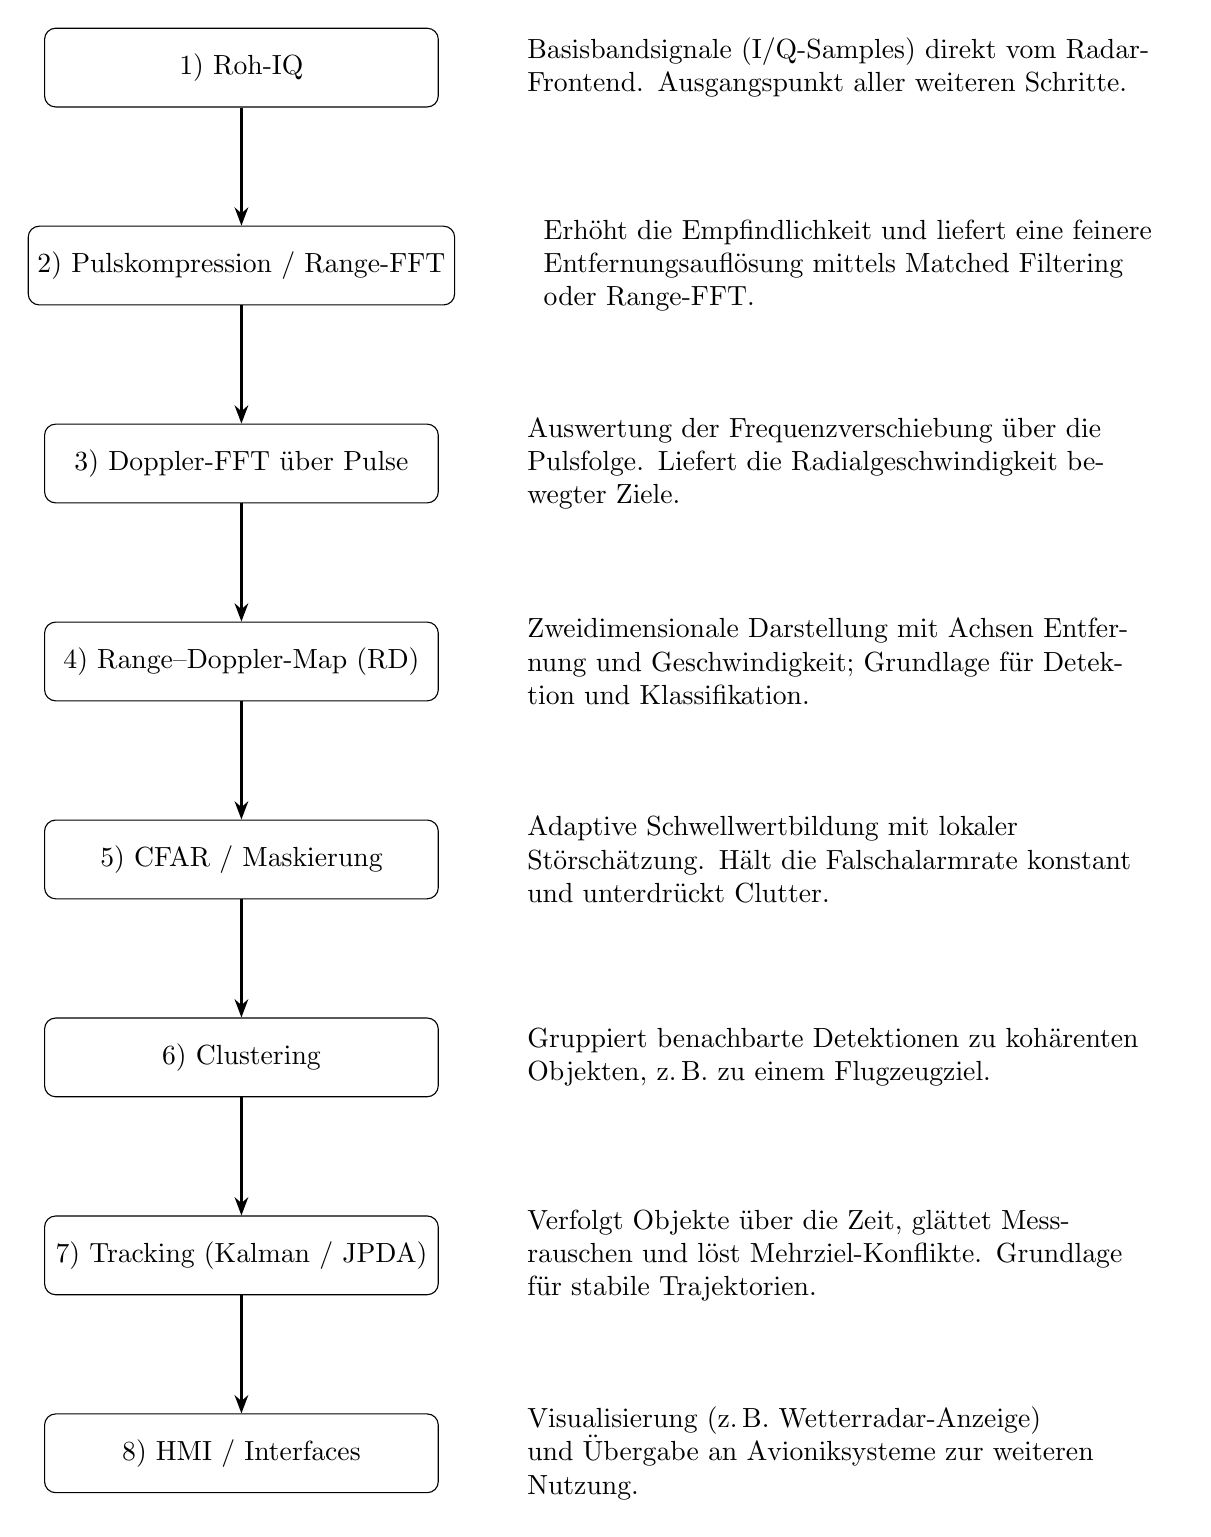
\begin{tikzpicture}[node distance=1.5cm]
  % Hauptkette
  \node[block] (raw) {1) Roh-IQ};
  \node[explain, right=1cm of raw] {Basisbandsignale (I/Q-Samples) direkt vom Radar-Frontend. Ausgangspunkt aller weiteren Schritte.};

  \node[block, below=of raw] (range) {2) Pulskompression / Range-FFT};
  \node[explain, right=1cm of range] {Erhöht die Empfindlichkeit und liefert eine feinere Entfernungsauflösung mittels Matched Filtering oder Range-FFT.};

  \node[block, below=of range] (doppler) {3) Doppler-FFT über Pulse};
  \node[explain, right=1cm of doppler] {Auswertung der Frequenzverschiebung über die Pulsfolge. Liefert die Radialgeschwindigkeit bewegter Ziele.};

  \node[block, below=of doppler] (rdmap) {4) Range–Doppler-Map (RD)};
  \node[explain, right=1cm of rdmap] {Zweidimensionale Darstellung mit Achsen Entfernung und Geschwindigkeit; Grundlage für Detektion und Klassifikation.};

  \node[block, below=of rdmap] (cfar) {5) CFAR / Maskierung};
  \node[explain, right=1cm of cfar] {Adaptive Schwellwertbildung mit lokaler Störschätzung. Hält die Falschalarmrate konstant und unterdrückt Clutter.};

  \node[block, below=of cfar] (cluster) {6) Clustering};
  \node[explain, right=1cm of cluster] {Gruppiert benachbarte Detektionen zu kohärenten Objekten, z.\,B. zu einem Flugzeugziel.};

  \node[block, below=of cluster] (track) {7) Tracking (Kalman / JPDA)};
  \node[explain, right=1cm of track] {Verfolgt Objekte über die Zeit, glättet Messrauschen und löst Mehrziel-Konflikte. Grundlage für stabile Trajektorien.};

  \node[block, below=of track] (hmi) {8) HMI / Interfaces};
  \node[explain, right=1cm of hmi] {Visualisierung (z.\,B. Wetterradar-Anzeige) und Übergabe an Avioniksysteme zur weiteren Nutzung.};

  % Verbindungen Hauptkette
  \draw[arrow] (raw) -- (range);
  \draw[arrow] (range) -- (doppler);
  \draw[arrow] (doppler) -- (rdmap);
  \draw[arrow] (rdmap) -- (cfar);
  \draw[arrow] (cfar) -- (cluster);
  \draw[arrow] (cluster) -- (track);
  \draw[arrow] (track) -- (hmi);
\end{tikzpicture}

\subsection{Detektion \& CFAR}
\begin{itemize}
  \item Ein Radar empfängt neben echten Zielen immer auch Rauschen, Clutter und Störsignale.
        Daher muss entschieden werden, ob das Echo ein echtes Ziel oder nur Zufall bzw.\ Clutter ist.
        Bei zu niedrigem Schwellenwert steigen zwar die Treffer, aber auch die Fehlalarme;
        bei zu hohem Schwellenwert sinken Fehlalarme, schwache Ziele gehen verloren.
  \item \textbf{Funktionsweise CFAR:}
        \begin{enumerate}
          \item Einteilung in Reichweitenzellen (Range Bins).
          \item Lokale Schätzung der Stör- bzw.\ Clutterleistung (z.\,B.\ Mittelung der Nachbarzellen).
          \item Adaptiver Schwellenwert, der die lokale Falschalarmrate konstant hält.
          \item Überschreitung der Schwelle $\Rightarrow$ Detektion eines Ziels.
        \end{enumerate}
  \item \textbf{Performancegrößen}: Entdeckungswahrscheinlichkeit (Pd), Falschalarmwahrscheinlichkeit (Pfa), ROC-Kurve als Trade-off-Darstellung.
\end{itemize}

\subsection{Auflösungen und Messfehler}
\begin{itemize}
  \item \textbf{Entfernungsauflösung}: Wie nahe zwei Ziele in Reichweite beieinanderliegen dürfen, um getrennt zu erscheinen;
        bestimmt durch Puls- und Signalbandbreite.
  \item \textbf{Geschwindigkeitsauflösung}: Kleinste unterscheidbare Relativgeschwindigkeit; geprägt durch Beobachtungszeit
        und Anzahl der ausgewerteten Pulse.
  \item \textbf{Winkelauflösung}: Fähigkeit, Ziele im Azimut oder in der Elevation zu trennen; abhängig von Antennenapertur und Verfahren der Winkelschätzung.
  \item \textbf{Reichweitenmessfehler}: Zufällige Abweichungen der gemessenen Entfernung; beeinflusst durch SNR und Pulskompression.
  \item \textbf{Geschwindigkeitsmessfehler}: Unsicherheit in der Doppler-Schätzung; abhängig von SNR, Beobachtungsdauer und Senderstabilität.
  \item \textbf{Winkelmessfehler}: Abweichung zwischen gemessenem und tatsächlichem Zielwinkel; abhängig von SNR, Antennengröße und Verfahren.
\end{itemize}

\subsection{Typische Trade-offs}
\begin{tabular}{p{0.3\textwidth} p{0.65\textwidth}}
\textbf{Reichweite vs.\ Auflösung} & Mehr Bandbreite verbessert die Entfernungsauflösung, erhöht aber Rauschbandbreite, Datenrate und Systemkomplexität. \\[0.5em]
\textbf{PRF-Wahl} & Niedrige PRF begünstigt große unambige Reichweite, erschwert aber unambige Geschwindigkeitsmessung; hohe PRF umgekehrt. Staggered/Multiple PRFs verringern Ambiguitäten, erhöhen jedoch Verarbeitungsaufwand. \\[0.5em]
\textbf{Winkelauflösung vs.\ Antennengröße} & Schmalere Beams (höhere Frequenz, größere Apertur, Mehrkanal/AESA) trennen Ziele besser, steigern aber Kosten, Leistungsaufnahme und Integrationsaufwand. \\[0.5em]
\textbf{CPI-Länge} & Längere Beobachtung verbessert Dopplerauflösung und Empfindlichkeit, erhöht aber Latenz und kann bei stark manövrierenden Zielen zu Unschärfe führen. \\[0.5em]
\textbf{Zeit–Frequenz–Unschärfe} & Kurze Signale lokalisieren Ereignisse gut in der Zeit (gut für Reichweite), verlieren aber Frequenzpräzision (schlechter für Geschwindigkeit); lange Signale umgekehrt. \\[0.5em]
\textbf{Detektionsschwelle vs.\ Fehlalarme} & Niedriger Schwellenwert steigert die Entdeckungswahrscheinlichkeit, aber auch die Falschalarmrate; höherer Schwellenwert reduziert Fehlalarme, kann schwache Ziele verpassen. CFAR gleicht dies adaptiv aus. \\[0.5em]
\textbf{Clutter-Unterdrückung vs.\ Zielerhalt} & Aggressive Filterung (z.\,B.\ MTI, Wettermasken) reduziert Störungen, riskiert aber langsame oder schwache Ziele zu dämpfen. \\[0.5em]
\textbf{Datenrate/Kompression vs.\ Informationsgehalt} & Hohe Abtastraten, viele Kanäle und feine Raster liefern reichhaltige RD(A)-Daten, treiben aber Schnittstellenlast, Speicher und Latenz. Kompression/Dezimierung spart Ressourcen, verliert aber Details. \\[0.5em]
\textbf{Wellenform-Komplexität vs.\ Robustheit} & Komplexe, modulierte Wellenformen bieten bessere Auflösung und Anti-Jam-Eigenschaften, erhöhen aber Implementierungsaufwand und Empfindlichkeit gegenüber Modellfehlern. \\[0.5em]
\textbf{Abdeckungsrate vs.\ Verweilzeit} & Schnelles Scannen erhöht Volumenabdeckung und Aktualität, reduziert jedoch Verweilzeit pro Blickrichtung und damit SNR; längere Verweilzeiten erhöhen SNR, senken aber Abdeckungsrate. \\
\end{tabular}

\subsection{Leistungskennzahlen (System \& Messung)}
\begin{tabular}{p{0.3\textwidth} p{0.65\textwidth}}
\textbf{Entdeckungswahrscheinlichkeit (Pd)} & Wahrscheinlichkeit, dass ein tatsächlich vorhandenes Ziel erkannt wird; hoher Wert bedeutet zuverlässige Detektion. \\[0.5em]
\textbf{Falschalarmwahrscheinlichkeit (Pfa)} & Wahrscheinlichkeit, dass ein Ziel gemeldet wird, obwohl keines existiert (z.\,B.\ durch Rauschen oder Clutter). \\[0.5em]
\textbf{ROC-Kurve} & Zeigt den Zusammenhang zwischen Pd und Pfa; macht den Trade-off sichtbar. \\[0.5em]
\textbf{Messfehler (Range, Geschwindigkeit, Winkel)} & Zufällige Abweichungen zwischen gemessenen und wahren Werten; beeinflusst durch SNR, Integrationszeit und Systemstabilität. \\[0.5em]
\textbf{Update-Rate / Latenz} & Zeitliche Aktualisierung der Messungen; höhere Raten verbessern Situationsbewusstsein, können jedoch die Verweilzeit reduzieren. \\[0.5em]
\textbf{Verfügbarkeit / Zuverlässigkeit} & Fähigkeit des Systems, über lange Zeit stabil Daten zu liefern – trotz Störungen oder widriger Bedingungen. \\
\end{tabular}


\section{Radar – Grundlagen für Objektklassifizierung}

\subsection{Wichtige Datenpunkte für Objektklassifikation}
\begin{tabular}{p{0.35\textwidth} p{0.6\textwidth}}
\textbf{Reichweite (Entfernung)} & Basisinformation für die Position eines Objekts relativ zum Radar; zentral für Lagebestimmung und Tracking. \\[0.5em]
\textbf{Relativgeschwindigkeit (Doppler)} & Erkennt Bewegung auf das Radar zu oder davon weg. Wichtig, um bewegte von statischen Objekten zu unterscheiden. \\[0.5em]
\textbf{Winkel (Azimut/Elevation)} & Richtung, aus der das Echo kommt. Unerlässlich für räumliche Lokalisierung und die Trennung mehrerer Ziele. \\[0.5em]
\textbf{Radar Cross Section (RCS)} & Stärke der Reflexion, abhängig von Größe, Material und Geometrie des Objekts; hilfreich für Typ- und Größenindizien. \\[0.5em]
\textbf{Doppler-Signatur / Mikrodoppler} & Feinstruktur durch bewegte Teile (z.\,B.\ Rotorblätter, Flügelschlag); liefert starke Trennmerkmale. \\[0.5em]
\textbf{Zeitliche Historie / Tracks} & Trajektorien über mehrere Messzyklen machen Verhalten sichtbar (z.\,B.\ stabile Flugbahn vs.\ flatternde Bewegung). \\[0.5em]
\textbf{Spektrale Eigenschaften der Echos} & Verteilung der Rückstreuung über Frequenz oder Polarisation kann Material- und Strukturhinweise geben. \\[0.5em]
\textbf{Clutter-Kontext} & Einordnung des Objekts im Umfeld: Bodenclutter, Wetter oder Seeoberfläche beeinflussen die Klassifikationssicherheit. \\[0.5em]
\textbf{SNR und Qualitätsmetriken} & Signal-Rausch-Verhältnis, CFAR-Maske, lokale Störschätzung; entscheidend, um unsichere Messungen korrekt zu gewichten. \\[0.5em]
\textbf{Sensor-/Modus-Metadaten} & Hinweise zu Wellenform, PRF, Antennen-Aspect oder Scanmodus helfen, Merkmale richtig zu interpretieren. \\[0.5em]
\textbf{Konsistenz über Zeit} & Persistenz, Aussetzer, Track-Confidence und Plausibilitätschecks (kinematische Grenzen) erhöhen die Robustheit. \\
\end{tabular}

\section{Merksätze zu Radar-Grundlagen und Objektklassifizierung}

\subsection{Radar-Grundlagen – wichtigste Merksätze}
\begin{itemize}
  \item \textbf{Physik zuerst:} Das Signal-Rausch-Verhältnis setzt die Grenzen – alles Weitere baut darauf auf.
  \item \textbf{Qualität wandert nach unten:} Stabilität von Range–Doppler–Angle bestimmt die Qualität aller Folgeschritte.
  \item \textbf{PRF ist ein Hebel:} Wahl der Pulsfolge legt den Kompromiss zwischen Reichweite und Geschwindigkeitsmessung fest.
  \item \textbf{Bandbreite kostet:} Bessere Auflösung erhöht Datenrate, Rechenlast und Anforderungen an Hardware.
  \item \textbf{Antenne = Winkel:} Größere Apertur oder elektronisches Schwenken verbessert Winkeltrennung, aber treibt Komplexität und Energiebedarf.
  \item \textbf{Beobachtungszeit vs.\ Latenz:} Längere Integrationszeiten schärfen Doppler, erhöhen aber Latenz und Bewegungsunschärfe.
  \item \textbf{CFAR steuert Falschalarmrate:} Zu niedrige Schwellen erzeugen Fehlalarme, zu hohe verpassen schwache Ziele.
  \item \textbf{Clutter ist der Hauptgegner:} Filter aggressiv genug wählen, ohne langsame oder schwache Ziele zu unterdrücken.
  \item \textbf{Mehrwege und Atmosphäre machen Geister:} Tracking und Konsistenzprüfungen enttarnen Scheinziele.
  \item \textbf{Koexistenz beachten:} Betrieb neben SSR/ADS-B, Funk- und Navigationsdiensten erfordert robuste Störfestigkeit.
  \item \textbf{Kalibrierung hält Systeme ehrlich:} Regelmäßige Checks und Health-Monitoring sichern Vergleichbarkeit und verhindern Drift.
  \item \textbf{Metadaten sind Gold:} Modus-, PRF- und Antenneninformationen gehören in die Daten, damit Auswertungen interpretierbar bleiben.
\end{itemize}

\subsection{Objektklassifizierung – wichtigste Merksätze}
\begin{itemize}
  \item \textbf{Stabilität vor KI:} Saubere Detektion, verlässliche RD/RDA-Daten und stabile Tracks sind die Basis guter Klassifikation.
  \item \textbf{Zeit schlägt Einzelbild:} Sequenzen und Trajektorien glätten Rauschen und offenbaren Muster besser als Einzelscans.
  \item \textbf{Mikrodoppler als Fingerabdruck:} Rotor- und Flügelschlag-Signaturen trennen Drohnen, Helikopter und Vögel – abhängig von SNR und Aspekt.
  \item \textbf{Quality-in-the-loop:} SNR, CFAR-Masken, Clutter- und Jamming-Flags als zusätzliche Eingabekanäle erhöhen Robustheit.
  \item \textbf{Offene Welt akzeptieren:} Eine \emph{Unknown}-Option und OOD-Detektion sind Pflicht – lieber aussetzen als falsch sicher sein.
  \item \textbf{Konfidenz muss stimmen:} Kalibrierte Wahrscheinlichkeiten und klare Abstain-Schwellen sind wichtiger als maximale Top-1-Quote.
  \item \textbf{Physik hilft:} Physikgeleitete Merkmale (z.\,B.\ kinematische Plausibilität, Spektralbreite, RCS-Trends) stabilisieren datengetriebene Modelle.
  \item \textbf{Szenariodeckung vor „Overall-Accuracy“:} Leistung immer nach SNR, Entfernung, Aspekt und Umgebung berichten – sonst täuscht Mittelung.
  \item \textbf{Splits ohne Leckage:} Trainings-/Testtrennung nach Szenarien (Standorte, Aspekte, Wetterlagen) verhindert zu optimistische Ergebnisse.
  \item \textbf{HMI klärt Erwartungen:} Anzeige von Top-k, Konfidenz und OOD/Qualitätsflags verhindert Fehlinterpretationen im Betrieb.
  \item \textbf{Vorverarbeitung prägt Merkmale:} Wahl von CFAR, Filterung und Normalisierung bestimmt, was das Modell überhaupt „sehen“ kann.
  \item \textbf{Robust denken:} Klassifikation muss mit Clutter, RFI und sporadischen Aussetzern umgehen – Fallbacks gehören zum Design.
\end{itemize}








\chapter{Sicherheit in der Luftfahrt}
\textbf{Sicherheit verstehen bedeutet, Risiken zu verstehen.}\\
Sicherheit (Safety) ist die Freiheit von unvertretbaren Risiken; Risiko bemisst sich über Eintrittswahrscheinlichkeit und Schadensschwere.

\section{Sicherheit – Grundlagen}

\subsection{Begriffsabgrenzung: Safety vs. Security}
Safety = Schutz vor unbeabsichtigten Fehlern/Versagen. \\
Security = Schutz vor absichtlichen Angriffen.\\

\subsection{Risikobegriffe und Schutzziele}
Risiko beschreibt die Kombination aus \emph{Schweregrad} einer möglichen Auswirkung und ihrer \emph{Eintrittswahrscheinlichkeit}. 
Beide werden gemeinsam (z.\,B. in einer Risikomatrix) bewertet, um ein \emph{tolerierbares Restrisiko} festzulegen. 
Ziel ist, Risiken durch geeignete Maßnahmen so weit zu mindern, dass sie akzeptabel sind (ALARP-Prinzip: as low as reasonably practicable).

\paragraph{Schutzziele (Safety Goals).}
Aus der Bewertung werden klare Schutzziele abgeleitet: Sie beschreiben, welche gefährlichen Zustände verhindert bzw.\ auf welche Weise sie beherrscht werden müssen (z.\,B.\ definierte Fallback-Zustände, Grenzen für Fehlalarme und Ausfälle).

\paragraph{Abgeleitete Sicherheitsanforderungen.}
Die Schutzziele werden in überprüfbare Anforderungen überführt (z.\,B.\ Reaktionszeiten, Verfügbarkeiten, Fehlertoleranz). 
Diese Anforderungen sind rückverfolgbar zu den identifizierten Risiken und bilden die Grundlage für Verifikation und Validierung.

\paragraph{Risikominderungsmaßnahmen.}
Maßnahmen lassen sich typischerweise in drei Kategorien gliedern:
\begin{itemize}
  \item \textbf{Präventiv} (Fehler vermeiden): robuste Architektur, Redundanz, Partitionierung.
  \item \textbf{Detektierend} (Fehler erkennen): Überwachung, Plausibilitätsprüfungen, Alarme.
  \item \textbf{Korrektiv} (Fehler beherrschen): Fallbackmodus, sichere Abschaltung. 
\end{itemize}

\paragraph{Akzeptanzkriterien und Nachweis.}
Akzeptanzkriterien definieren, wann ein Restrisiko als tragbar gilt. Die Erfüllung wird durch Analysen, Tests und Inspektionen nachgewiesen und über den gesamten Lebenszyklus dokumentiert (Traceability von Gefährdung $\rightarrow$ Schutzziel $\rightarrow$ Anforderung $\rightarrow$ Nachweis).
Das ist essentiell für die Entwicklung von Komponenten und muss angemssen Dokumentiert werden in der Safety-Argumentation.

\subsection{Safety-Argumentation (Assurance Case)}
Ein \emph{Assurance Case} begründet systematisch und nachvollziehbar, dass ein System unter definierten Einsatzbedingungen \emph{sicher genug} ist. 
Er verbindet nachvollziehbare Behauptungen (Claims/Goals) mit einer transparenten Argumentationsstruktur, dokumentierten Annahmen und geeigneten Nachweisen (Analysen, Tests).

\paragraph{Zweck und Grundprinzip.}
Ziel ist eine prüfbare Argumentation: 
\begin{itemize}
    \item \emph{Was} wird behauptet (Claim)
    \item \emph{warum} ist das plausibel (Strategie/Begründung)
    \item \emph{unter welchen Bedingungen} gilt es (Kontext/Annahmen)
    \item \emph{wodurch} wird es gestützt (Evidenz)
\end{itemize}
Die Argumentation ist der Kern der Dokumentation und dient als Nachweis das etwas sicher genug ist.

\subsection{Gefahrenanalyse und Risikoermittlung}
Ziel der Gefahrenanalyse ist es, mögliche Gefährdungen früh zu erkennen, ihr Risiko grob einzuordnen und wirksame Gegenmaßnahmen abzuleiten. Das Ergebnis ist eine priorisierte Liste von Risiken mit klaren Safety-Zielen und abgeleiteten Anforderungen – und ein Plan, wie diese nachgewiesen werden.

\paragraph{Ablauf in Kurzform.}
\begin{enumerate}
  \item \textbf{Sammeln:} Mögliche Gefährdungen identifizieren (Technik, Mensch, Umfeld, Betrieb).
  \item \textbf{Einordnen:} Schweregrad und Eintrittswahrscheinlichkeit bewerten (Risikomatrix).
  \item \textbf{Maßnahmen ableiten:} Präventiv, detektierend, korrektiv.
  \item \textbf{Anforderungen festlegen:} Messbar, überprüfbar, rückverfolgbar.
  \item \textbf{Pflegen:} Über den Lebenszyklus regelmäßig aktualisieren.
\end{enumerate}

\paragraph{Methoden (kurz erklärt).}
\begin{itemize}
  \item \textbf{Hazard Identification (HAZID):} Strukturierte Sammlung von Gefährdungen per Workshops, Checklisten und Erfahrungswissen. Ergebnis: Hazard-Liste mit Ursachen, Wirkungen und Annahmen.
  \item \textbf{FMEA/FMECA:} \emph{Bottom-up} auf Komponenten- oder Funktionsebene: Welche Ausfallarten gibt es, was passiert dann, wie wird es entdeckt? FMECA ergänzt eine Kritikalitätsbewertung, um Prioritäten zu setzen.
  \item \textbf{Fault Tree Analysis (FTA):} \emph{Top-down} vom unerwünschten Ereignis (z.\,B. Verlust der Warnfunktion) zu seinen Ursachen. Eignet sich, Ketten/Wechselwirkungen sichtbar zu machen.
  \item \textbf{STPA:} Systemtheoretischer Ansatz: Welche \emph{unsicheren Steueraktionen} und Rahmenbedingungen führen zu Gefährdungen – inkl.\ Software, HMI und Prozeduren, nicht nur Hardware.
\end{itemize}

\subsection{Architekturprinzipien der funktionalen Sicherheit}
Ziel dieser Prinzipien ist es, Risiken durch die Systemarchitektur zu senken: Fehler sollen gar nicht erst wirken, früh erkannt oder sicher beherrscht werden. Im Fokus stehen klare Strukturen, vorhersehbares Verhalten und beherrschte Degradation statt Überraschungen.

\paragraph{Redundanz und Diversität/Dissimilarität}
\textbf{Redundanz} bedeutet, kritische Funktionen mehrfach vorzuhalten (z.\,B.\ zwei unabhängige Empfangsketten oder Stromversorgungen), sodass beim Ausfall einer Instanz die andere übernimmt.
\textbf{Diversität/Dissimilarität} ergänzt dies durch bewusst unterschiedliche Ausprägungen (z.\,B.\ verschiedene Hardware/Software oder unterschiedliche Algorithmen), damit ein gemeinsamer Fehler nicht alle Kanäle gleichzeitig trifft.
\emph{Beispiel:} Zwei unabhängige Radarpfade, davon einer mit alternativer Signalverarbeitung.

\paragraph{Trennung/Partitionierung}
Trennung verhindert Fehlerfortpflanzung: sicherheitskritische Anteile laufen räumlich und zeitlich isoliert von weniger kritischen Funktionen. Partitionierung (z.\,B.\ per Betriebssystem mit Zeit-/Speichertrennung) stellt sicher, dass ein Fehler in einer Partition keine andere beeinträchtigt.
\emph{Beispiel:} Klassifikations-KI in einer strikt begrenzten Partition; Kerndetektion und HMI getrennt.

\paragraph{Fail-Safe vs.\ Fail-Operational}
\textbf{Fail-Safe} bedeutet, bei einem Fehler in einen definiert sicheren Zustand zu wechseln (z.\,B.\ Abschalten einer Funktion, klare Warnung, konservatives Verhalten).
\textbf{Fail-Operational} bedeutet, trotz eines Fehlers die Funktion weiter bereitzustellen – ggf.\ in degradiertem Modus –, weil ein Abbruch riskanter wäre.
\emph{Beispiel:} Bei Sensorausfall Umschalten auf redundanten Kanal (fail-operational); bei inkonsistenten Daten Anzeige eines geprüften Minimalbildes mit Warnhinweis (fail-safe).

\paragraph{Deterministische Kommunikation}
Kommunikation und Zeitverhalten müssen vorhersagbar sein: feste oder begrenzte Latenzen, kontrollierter Jitter, klare Prioritäten und synchronisierte Uhren. So lassen sich Worst-Case-Reaktionszeiten planen und nachweisen.
\emph{Beispiel:} Zeitgesteuerte Übertragung sicherheitskritischer Radar-Updates mit garantierter maximaler Verzögerung.

\subsection{Verifikation und Validierung (V\&V)}
Ziel von V\&V ist es nachzuweisen, dass die Anforderungen korrekt, vollständig und erfüllt sind – und dass das System im vorgesehenen Einsatz \emph{das Richtige} tut.
\textbf{Verifikation} fragt: „Haben wir das Produkt richtig gebaut?“
\textbf{Validierung} fragt: „Haben wir das richtige Produkt gebaut?“

Getestet wird auf verschiedenen Ebenen: von Einheiten über Integration bis hin zu System- und Abnahme-Tests. 
Dieses Schichtenprinzip prüft Schnittstellen und stellt das Zusammenspiel zwischen Komponent und Gesammsystem sicher. 
Unabhängige Reviews erhöhen zudem die Beweiskraft, klare Kriterien machen Ergebnisse bewertbar, und Traceability verknüpft Anforderungen, Tests und Resultate. \\
Wichtig ist: Belege zählen! Ohne dokumentierte Ergebnisse gibt es keinen Nachweis.


\subsection{Lebenszyklus}
Safety muss über den gesamten Lebenszyklus gewährleistet sein.\\
Es genügt nicht, wenn die verbauten Komponenten zu Beginn sicher sind. Z.B. müssen Umgebungsveränderungen berücksichtigt werden 
und gegebenenfalls Sofwareupdates oder Reparaturen eingeplant werden.

\subsection{Human Factors und HMI}
In der Entwicklung muss der Faktor Mensch brücksichtigt werden.
Der Mensch ist eine potentielle Fehlerquelle und das Produkt muss für den Menschen sicher sein.

\subsection{Kurzhinweis zu Security}
Security-Vorfälle können Safety-Ziele gefährden und müssen daher bei Anforderungen, Design, etc. berücksichtigt werden. \\
Da der Fokus auf Safety liegt, wird Security nicht genauer durchleutet.


\section{Luftfahrt-spezifische Sicherheit}

\subsection{Regulatorischer Rahmen und Akteure}
\textit{Ziel:} Einordnung von EASA/FAA, Zulassungswegen (z.\,B. TSO/ETSO, Part 21) und Rollen der Organisationen.

\subsection{Safety-Standards und Prozesse (Überblick)}
\textit{Ziel:} Welche Normfamilien den Safety-Prozess leiten.
\textit{Inhalt:} ARP4754A (Systementwicklung), ARP4761A (Safety-Analysen), DO-178C (Software), DO-254 (Hardware), DO-160 (Umwelteinflüsse).

\subsection{Development Assurance Levels (DAL)}
\textit{Ziel:} Zusammenhang von Hazard-Schweregrad und Entwicklungs-/Nachweisstrenge.
\textit{Inhalt:} DAL A–E, Unabhängigkeit, Nachweisintensität, Auswirkungen auf Prozesse/Tests.

\subsection{Safety-Assessments im Entwicklungsfluss}
\textit{Ziel:} Wie Safety systematisch in die Entwicklung integriert wird.
\textit{Inhalt:} FHA (Functional Hazard Assessment), PSSA (Preliminary System Safety Assessment), SSA (System Safety Assessment),
CCA (Common Cause Analysis inkl. Zonal/Particular Risks); Inputs/Outputs und Verknüpfung zu Anforderungen.

\subsection{Architekturprinzipien in der Avionikpraxis}
\textit{Ziel:} Safety-fördernde Umsetzungen in realen Systemen.
\textit{Inhalt:} Partitionierung (z.\,B. zeit-/raumgetrennte Ausführung), deterministische Netzwerke (z.\,B. AFDX/TTEthernet), Zeit-Synchronisation,
Built-In Tests, Wartbarkeit/Fehlerisolierung.

\subsection{Verifikation/Validierung in der Luftfahrt}
\textit{Ziel:} Branchenspezifische Erwartungen an V\&V.
\textit{Inhalt:} Unabhängige Verifikation, Abdeckungsanforderungen (z.\,B. hohe Testtiefe), Nachweisarten und Compliance-Dokumente.

\subsection{Betrieb und Continuing Airworthiness}
\textit{Ziel:} Safety nach der Zulassung sichern.
\textit{Inhalt:} Vorkommnismeldungen, Service Bulletins/Airworthiness Directives, Patch-/Änderungsmanagement, Konfigurationskontrolle.

\subsection{Human Factors, SOPs und Training}
\textit{Ziel:} Safety in Betrieb und Bedienung verankern.
\textit{Inhalt:} Crew-/Maintenance-Training, klare SOPs, Umgang mit Degradations-/Fallback-Modi und Alarmen.

\subsection{Brücke zu KI/ML (Vorschau mit Safety-Fokus)}
\textit{Ziel:} Kurz ankündigen, wie die Safety-Grundsätze auf KI/ML angewendet werden (Kalibrierung, OOD/Abstain, Safety-Cage, Nachweise) – Details im KI-Kapitel.











\chapter{KI in der Luftfahrt}
\section{Use-Cases} 











\chapter{KI Sicherheit}
\section{Begriffe} 

\subsection{AI Safety}
= beherrschbares, verlässliches Verhalten (funktionale Sicherheit, Fehlertoleranz).

\subsection{AI Security}
= Schutz der KI vor Angriffen (Poisoning, Adversarial, Model Theft).

\subsection{Airworthiness Security}
= luftfahrtspezifische Security-Prozesse.




\section{Risiken}
Safety-Fehler (Fehlklassifikation, schlechte Kalibrierung, OOD-Blindheit) 
vs. Security-Angriffe (Jamming/DRFM auf Sensor-Ebene, Backdoors/Adversarial auf ML-Ebene).

\section{Design-Prinzipien}
\subsection{Safety}
Kalibrierung, Unsicherheits-Schätzung, Abstain/Unknown, Safety-Cage/Simplex, erklärbare Features.

\subsection{Security}
Daten-Governance, signierte Modelle/secure boot, OOD/Anomalie-Wächter, adversarial Training, Red-Team-Tests.

\section{Metriken und Evidenz}
ECE/Brier, OOD-Rate, adversarial Erfolgsrate, J/S-Robustheit, Traceability (Req <-> Test <-> Befund).











